\documentclass[11pt,preprint, authoryear]{elsarticle}

\usepackage{lmodern}
%%%% My spacing
\usepackage{setspace}
\setstretch{1.2}
\DeclareMathSizes{12}{14}{10}{10}

% Wrap around which gives all figures included the [H] command, or places it "here". This can be tedious to code in Rmarkdown.
\usepackage{float}
\let\origfigure\figure
\let\endorigfigure\endfigure
\renewenvironment{figure}[1][2] {
    \expandafter\origfigure\expandafter[H]
} {
    \endorigfigure
}

\let\origtable\table
\let\endorigtable\endtable
\renewenvironment{table}[1][2] {
    \expandafter\origtable\expandafter[H]
} {
    \endorigtable
}


\usepackage{ifxetex,ifluatex}
\usepackage{fixltx2e} % provides \textsubscript
\ifnum 0\ifxetex 1\fi\ifluatex 1\fi=0 % if pdftex
  \usepackage[T1]{fontenc}
  \usepackage[utf8]{inputenc}
\else % if luatex or xelatex
  \ifxetex
    \usepackage{mathspec}
    \usepackage{xltxtra,xunicode}
  \else
    \usepackage{fontspec}
  \fi
  \defaultfontfeatures{Mapping=tex-text,Scale=MatchLowercase}
  \newcommand{\euro}{€}
\fi

\usepackage{amssymb, amsmath, amsthm, amsfonts}

\def\bibsection{\section*{References}} %%% Make "References" appear before bibliography


\usepackage[round]{natbib}

\usepackage{longtable}
\usepackage[margin=2.3cm,bottom=2cm,top=2.5cm, includefoot]{geometry}
\usepackage{fancyhdr}
\usepackage[bottom, hang, flushmargin]{footmisc}
\usepackage{graphicx}
\numberwithin{equation}{section}
\numberwithin{figure}{section}
\numberwithin{table}{section}
\setlength{\parindent}{0cm}
\setlength{\parskip}{1.3ex plus 0.5ex minus 0.3ex}
\usepackage{textcomp}
\renewcommand{\headrulewidth}{0.2pt}
\renewcommand{\footrulewidth}{0.3pt}

\usepackage{array}
\newcolumntype{x}[1]{>{\centering\arraybackslash\hspace{0pt}}p{#1}}

%%%%  Remove the "preprint submitted to" part. Don't worry about this either, it just looks better without it:
\makeatletter
\def\ps@pprintTitle{%
  \let\@oddhead\@empty
  \let\@evenhead\@empty
  \let\@oddfoot\@empty
  \let\@evenfoot\@oddfoot
}
\makeatother

 \def\tightlist{} % This allows for subbullets!

\usepackage{hyperref}
\hypersetup{breaklinks=true,
            bookmarks=true,
            colorlinks=true,
            citecolor=blue,
            urlcolor=blue,
            linkcolor=blue,
            pdfborder={0 0 0}}


% The following packages allow huxtable to work:
\usepackage{siunitx}
\usepackage{multirow}
\usepackage{hhline}
\usepackage{calc}
\usepackage{tabularx}
\usepackage{booktabs}
\usepackage{caption}


\newenvironment{columns}[1][]{}{}

\newenvironment{column}[1]{\begin{minipage}{#1}\ignorespaces}{%
\end{minipage}
\ifhmode\unskip\fi
\aftergroup\useignorespacesandallpars}

\def\useignorespacesandallpars#1\ignorespaces\fi{%
#1\fi\ignorespacesandallpars}

\makeatletter
\def\ignorespacesandallpars{%
  \@ifnextchar\par
    {\expandafter\ignorespacesandallpars\@gobble}%
    {}%
}
\makeatother

\newlength{\cslhangindent}
\setlength{\cslhangindent}{1.5em}
\newenvironment{CSLReferences}%
  {\setlength{\parindent}{0pt}%
  \everypar{\setlength{\hangindent}{\cslhangindent}}\ignorespaces}%
  {\par}


\urlstyle{same}  % don't use monospace font for urls
\setlength{\parindent}{0pt}
\setlength{\parskip}{6pt plus 2pt minus 1pt}
\setlength{\emergencystretch}{3em}  % prevent overfull lines
\setcounter{secnumdepth}{5}

%%% Use protect on footnotes to avoid problems with footnotes in titles
\let\rmarkdownfootnote\footnote%
\def\footnote{\protect\rmarkdownfootnote}
\IfFileExists{upquote.sty}{\usepackage{upquote}}{}

%%% Include extra packages specified by user

%%% Hard setting column skips for reports - this ensures greater consistency and control over the length settings in the document.
%% page layout
%% paragraphs
\setlength{\baselineskip}{12pt plus 0pt minus 0pt}
\setlength{\parskip}{12pt plus 0pt minus 0pt}
\setlength{\parindent}{0pt plus 0pt minus 0pt}
%% floats
\setlength{\floatsep}{12pt plus 0 pt minus 0pt}
\setlength{\textfloatsep}{20pt plus 0pt minus 0pt}
\setlength{\intextsep}{14pt plus 0pt minus 0pt}
\setlength{\dbltextfloatsep}{20pt plus 0pt minus 0pt}
\setlength{\dblfloatsep}{14pt plus 0pt minus 0pt}
%% maths
\setlength{\abovedisplayskip}{12pt plus 0pt minus 0pt}
\setlength{\belowdisplayskip}{12pt plus 0pt minus 0pt}
%% lists
\setlength{\topsep}{10pt plus 0pt minus 0pt}
\setlength{\partopsep}{3pt plus 0pt minus 0pt}
\setlength{\itemsep}{5pt plus 0pt minus 0pt}
\setlength{\labelsep}{8mm plus 0mm minus 0mm}
\setlength{\parsep}{\the\parskip}
\setlength{\listparindent}{\the\parindent}
%% verbatim
\setlength{\fboxsep}{5pt plus 0pt minus 0pt}



\begin{document}



\begin{frontmatter}  %

\title{Replication: Identifying Aggregate Supply and Demand Shocks in
South Africa}

% Set to FALSE if wanting to remove title (for submission)




\author[Add1]{Samantha Scott}
\ead{20945043@sun.ac.za}





\address[Add1]{Stellenbosch University, Cape Town, South Africa}

\cortext[cor]{Corresponding author: Samantha Scott}


\vspace{1cm}


\begin{keyword}
\footnotesize{
Econometrics \sep Time Series \sep VAR \sep SVAR \sep Blanchard-Quah \\
\vspace{0.3cm}
}
\end{keyword}



\vspace{0.5cm}

\end{frontmatter}



%________________________
% Header and Footers
%%%%%%%%%%%%%%%%%%%%%%%%%%%%%%%%%
\pagestyle{fancy}
\chead{}
\rhead{}
\lfoot{}
\rfoot{\footnotesize Page \thepage}
\lhead{}
%\rfoot{\footnotesize Page \thepage } % "e.g. Page 2"
\cfoot{}

%\setlength\headheight{30pt}
%%%%%%%%%%%%%%%%%%%%%%%%%%%%%%%%%
%________________________

\headsep 35pt % So that header does not go over title




\hypertarget{introduction}{%
\section{Introduction}\label{introduction}}

The paper, \emph{Identifying aggregate supply and demand shocks in South
Africa}, is an application of a structural VAR method to identify supply
and demand shocks for the South African economy since the 1960s. The aim
of this paper is to replicate the paper by Du Plessis, Smit and
Sturzenegger (2008), with

\hypertarget{data}{%
\section{Data}\label{data}}

The data used is quarterly data from FRED, dating back to 1960 up until
2007. Unlike the original paper, the data used is not seasonally
adjusted. The variables used in the model are the first difference of
the log of GDP (\(y_t\)), the ratio of government consumption to GDP
(\(g_t\)), as well the real interest rate (\(r_t\)). \(r_t\) is
calculated using the monthly nominal interest rate as well as the
monthly CPI data. Below is the equation used to caluclate \(r_t\).

\[ r_t = ((1 + Avg(i_{mt-1}, i_{mt}, i_{mt+1}))/(1+(ln(CPI_{mt-2}) - ln(CPI_{mt+1}))) ^ 4 - 1)*100 \]
Figures 1, 2 and 3 represent the variables used. As seen in the
Appendix, when as Augmented Dickey-Fuller test is conducted, it is
evident that \(y_t\) is stationary, as the p-value is less than 0.05.
However, both \(g_t\) and \(r_t\) are non-stationary. In the original
paper (2007), \(r_t\) is stationary. This may be due to the data used
for this paper not being seasonally adjusted.

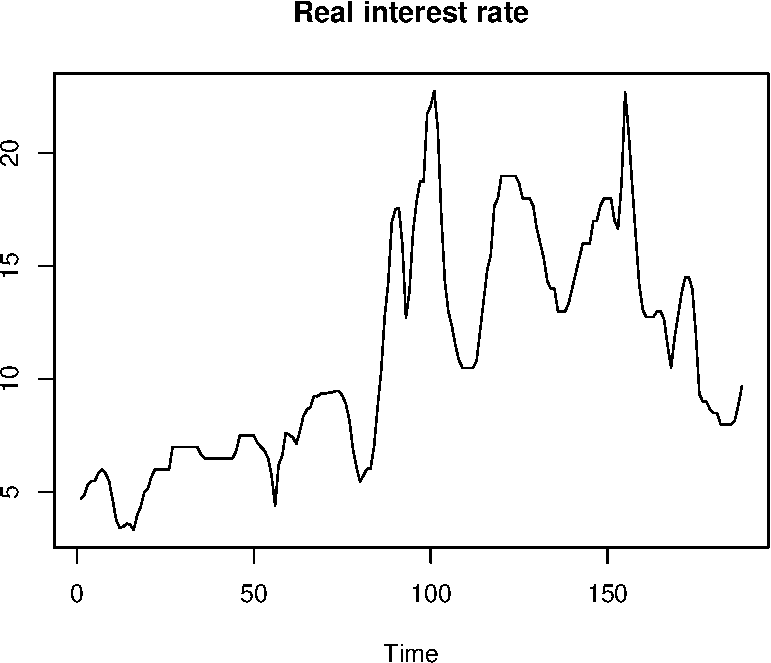
\includegraphics{TS_proj_files/figure-latex/unnamed-chunk-12-1.pdf}

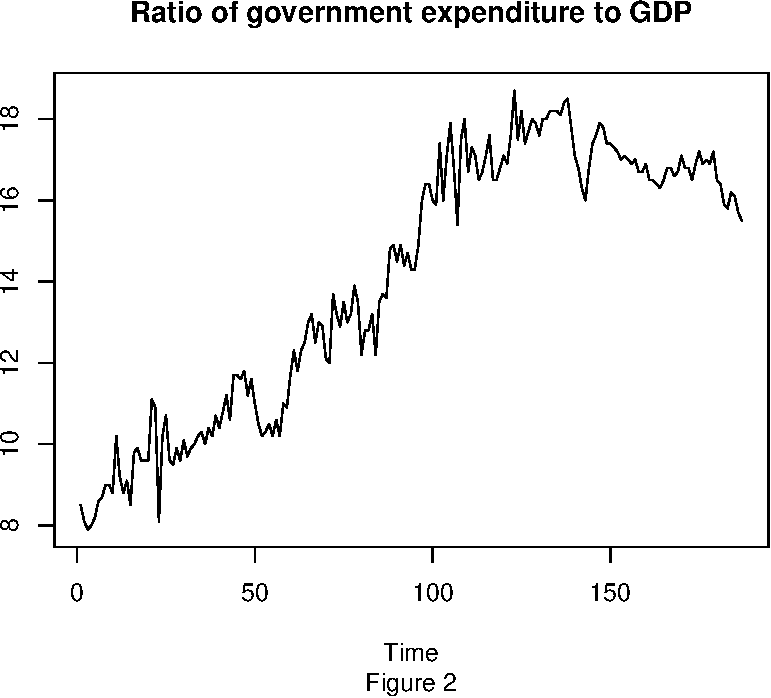
\includegraphics{TS_proj_files/figure-latex/unnamed-chunk-13-1.pdf}

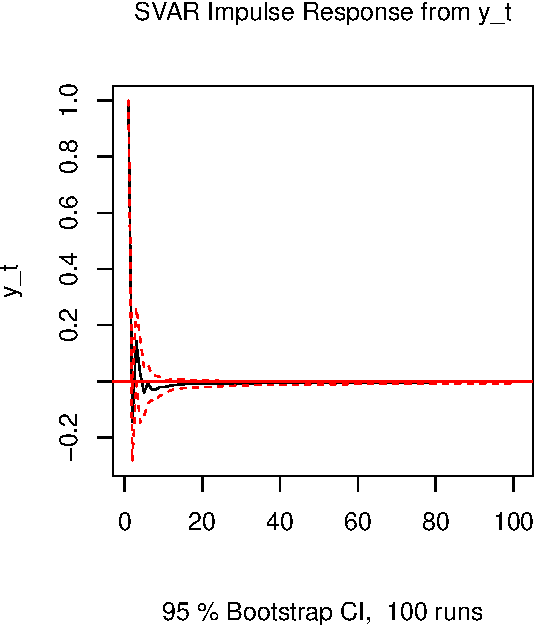
\includegraphics{TS_proj_files/figure-latex/unnamed-chunk-14-1.pdf}

\hypertarget{methodology}{%
\section{Methodology}\label{methodology}}

A structural VAR model is created to identify supply and demand shocks
for the South African economy since the 1960s. The demand the variables,
\(y_t\), \(g_t\) and \(r_t\) are proxies for a supply shock, a fiscal
shock and a monetary shock, respectively.

\hypertarget{results}{%
\section{Results}\label{results}}

The results of the model are presented as impulse response functions.

\hypertarget{impulse-response-of-real-gdp-for-each-of-the-identified-shocks}{%
\subsection{Impulse Response of real GDP for each of the identified
shocks}\label{impulse-response-of-real-gdp-for-each-of-the-identified-shocks}}

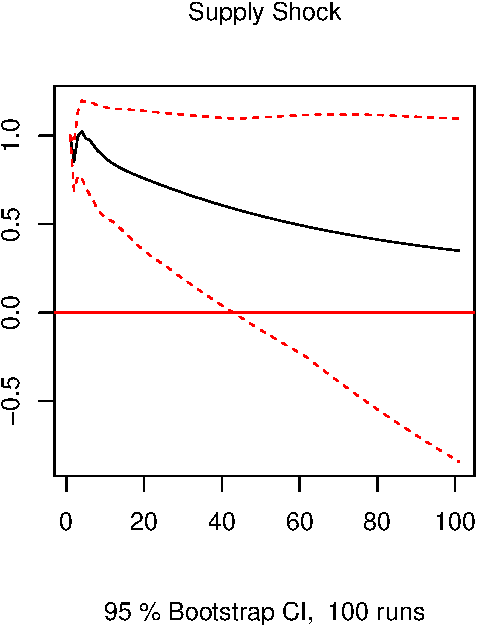
\includegraphics{TS_proj_files/figure-latex/unnamed-chunk-18-1.pdf}
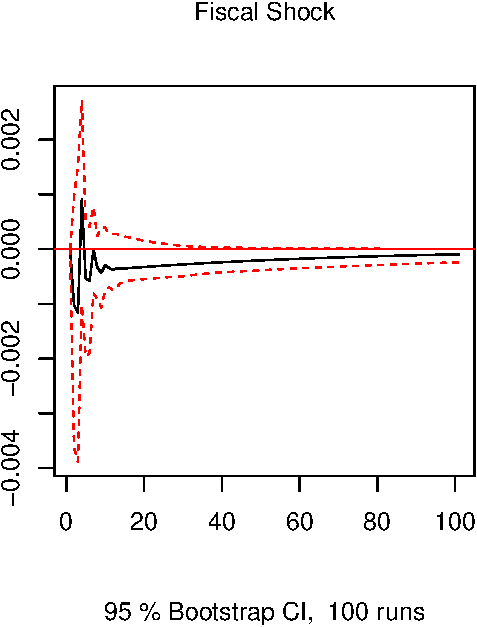
\includegraphics{TS_proj_files/figure-latex/unnamed-chunk-18-2.pdf}
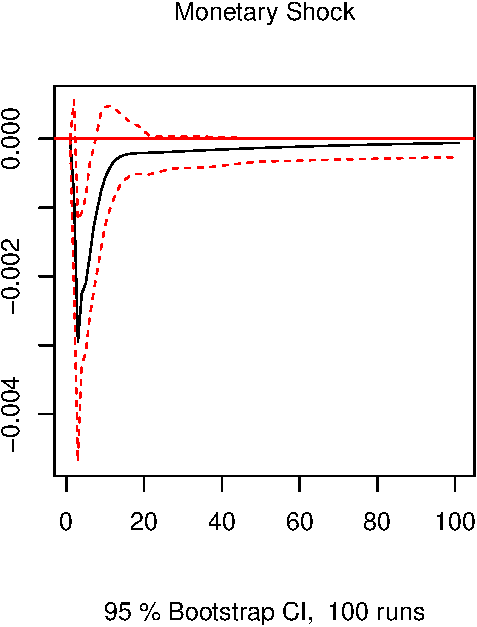
\includegraphics{TS_proj_files/figure-latex/unnamed-chunk-18-3.pdf}

\hypertarget{impulse-response-of-the-real-interest-rate-for-each-of-the-identified-shocks}{%
\subsection{Impulse Response of the real interest rate for each of the
identified
shocks}\label{impulse-response-of-the-real-interest-rate-for-each-of-the-identified-shocks}}

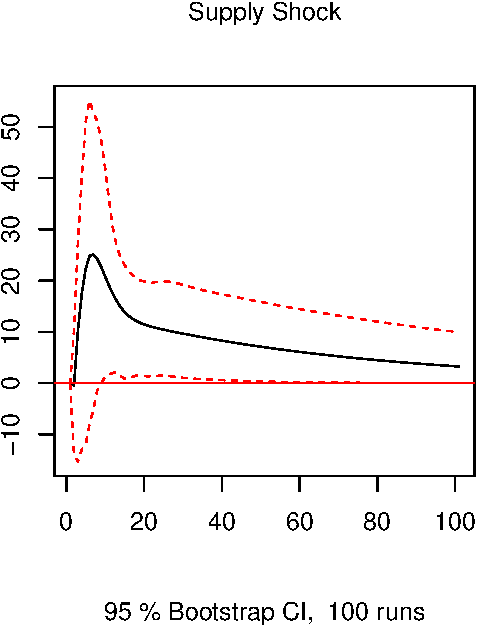
\includegraphics{TS_proj_files/figure-latex/unnamed-chunk-19-1.pdf}
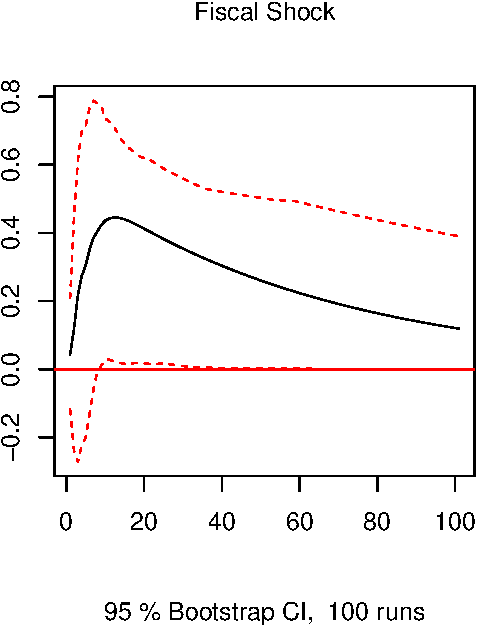
\includegraphics{TS_proj_files/figure-latex/unnamed-chunk-19-2.pdf}
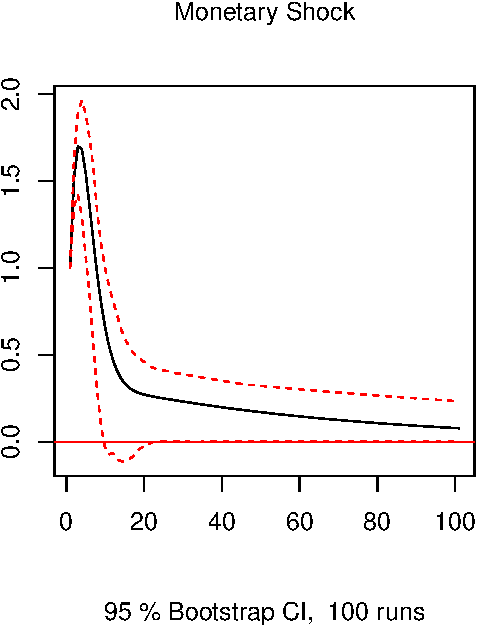
\includegraphics{TS_proj_files/figure-latex/unnamed-chunk-19-3.pdf}

\hypertarget{impulse-response-of-the-government-consumption-to-real-gdp-for-each-of-the-identified-shocks}{%
\subsection{Impulse Response of the government consumption to real GDP
for each of the identified
shocks}\label{impulse-response-of-the-government-consumption-to-real-gdp-for-each-of-the-identified-shocks}}

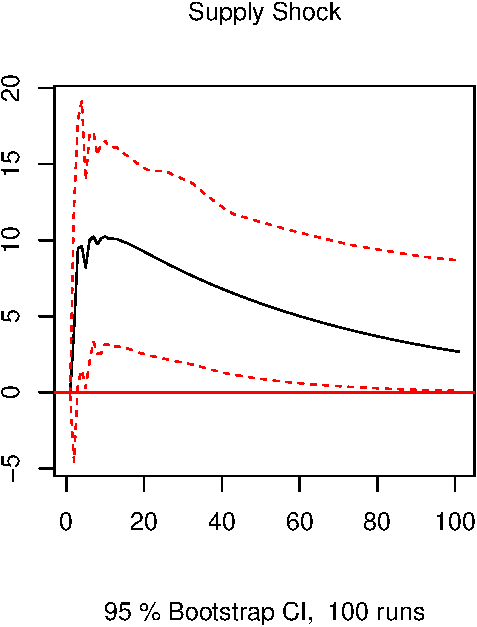
\includegraphics{TS_proj_files/figure-latex/unnamed-chunk-20-1.pdf}
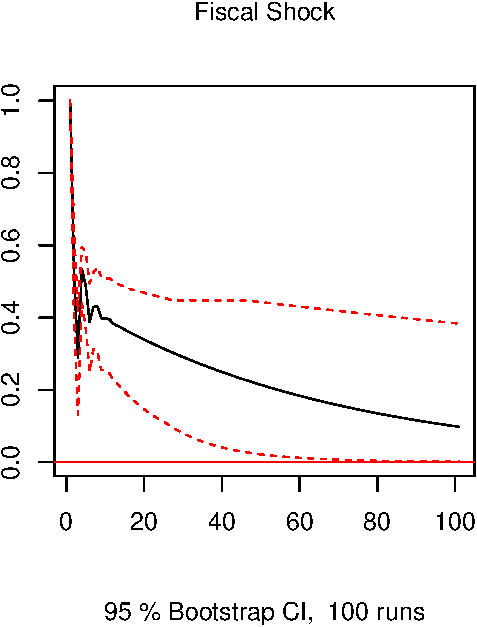
\includegraphics{TS_proj_files/figure-latex/unnamed-chunk-20-2.pdf}
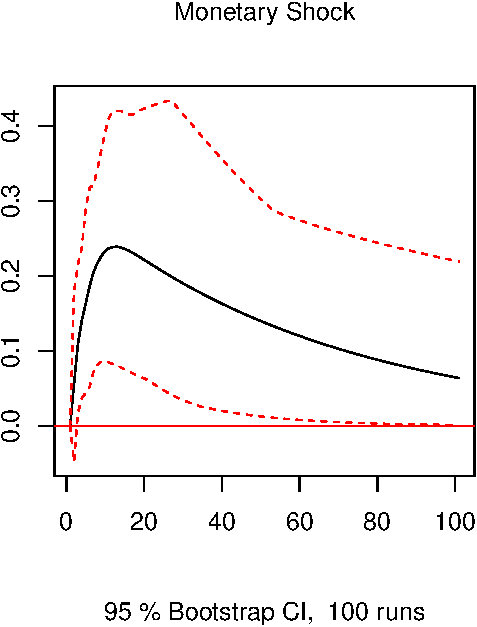
\includegraphics{TS_proj_files/figure-latex/unnamed-chunk-20-3.pdf}

\hypertarget{variance-decomposition}{%
\subsection{Variance Decomposition}\label{variance-decomposition}}

``The variance decomposition indicates the amount of information each
variable contributes to the other variables in the autoregression. It
determines how much of the forecast error variance of each of the
variables can be explained by exogenous shocks to the other variables.''

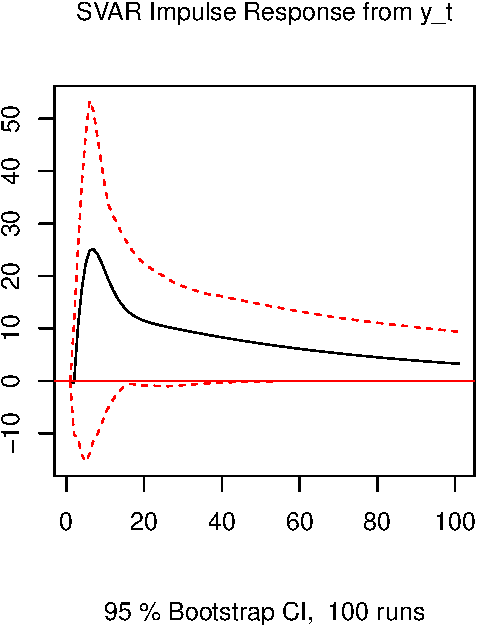
\includegraphics{TS_proj_files/figure-latex/unnamed-chunk-21-1.pdf}

\hypertarget{robustness-checks}{%
\section{Robustness Checks}\label{robustness-checks}}

\hypertarget{residuals}{%
\subsection{Residuals}\label{residuals}}

checking if residuals are white noise

``The residuals are the differences between the fitted model and the
data. In a signal-plus-white noise model, if you have a good fit for the
signal, the residuals should be white noise.''

Below is a check for residuals for the \(y_t\) variable. This helps to
determine whether the residual are white noise.

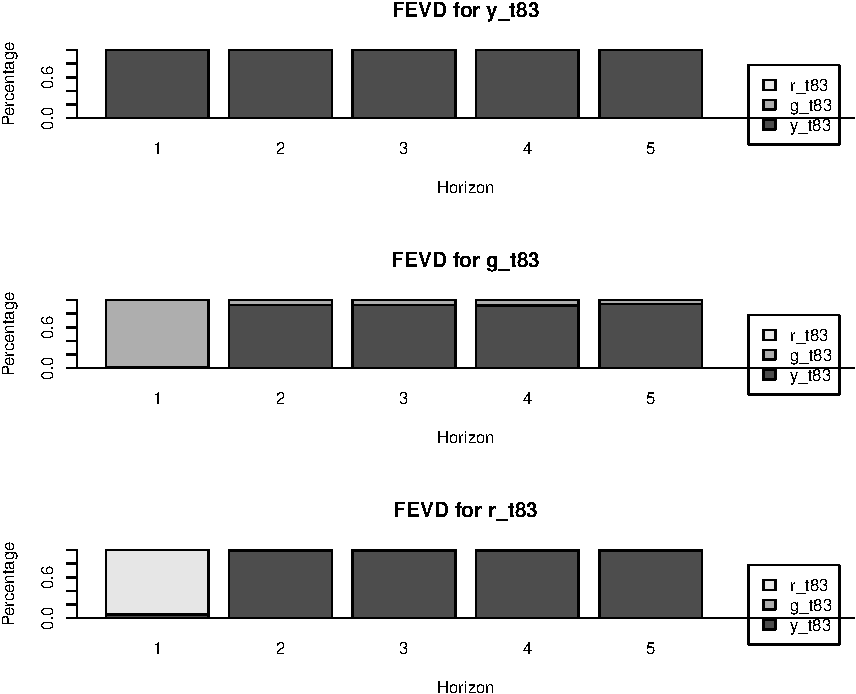
\includegraphics{TS_proj_files/figure-latex/unnamed-chunk-22-1.pdf}

Below is a check for residuals for the \(g_t\) variable.

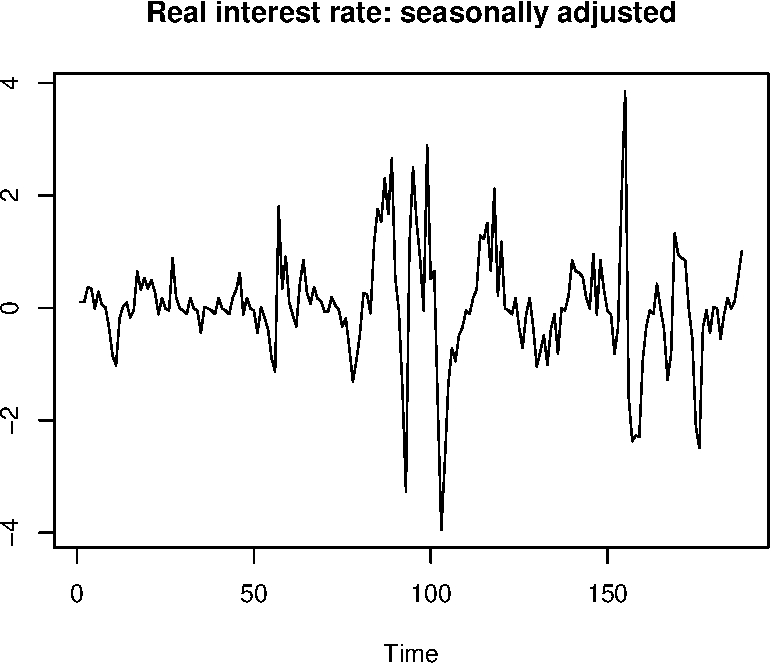
\includegraphics{TS_proj_files/figure-latex/unnamed-chunk-23-1.pdf}

Below is a check for residuals for the \(r_t\) variable.

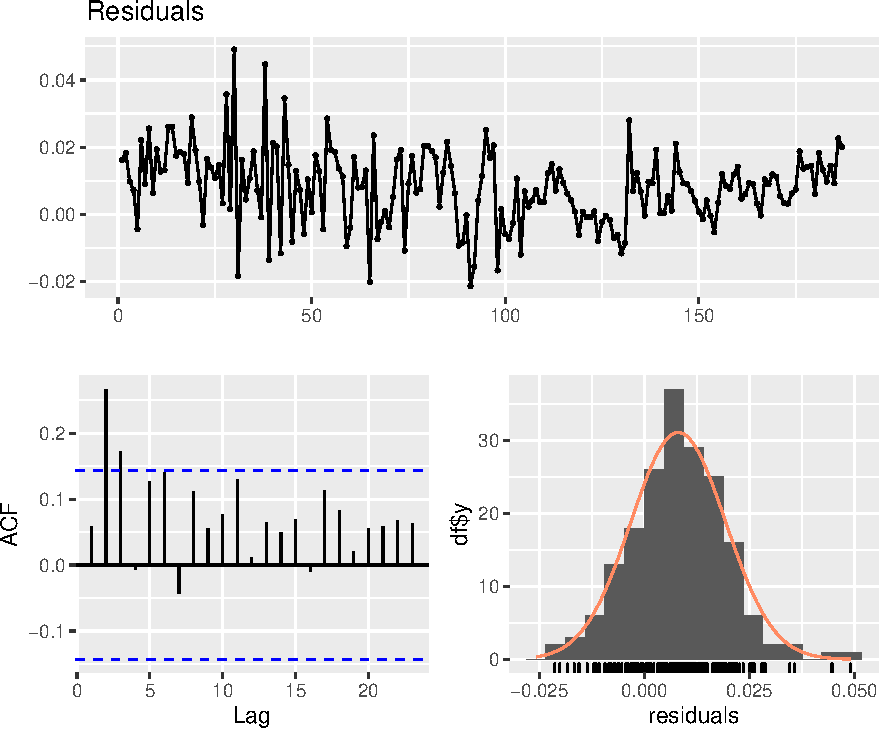
\includegraphics{TS_proj_files/figure-latex/unnamed-chunk-24-1.pdf}

\hypertarget{lag-selection}{%
\subsection{Lag Selection}\label{lag-selection}}

``Lütkepohl (1993) indicates that overfitting (selecting a higher order
lag length than the true lag length) causes an increase in the
mean-squareforecast errors of the VAR and that underfitting the lag
length often generates autocorrelated errors.''

The first set of Impulse Response Functions below are presented using a
second SVAR model, where the number of lags selected is 6.

\hypertarget{reduced-sample-from-last-quarter-1983}{%
\subsection{Reduced Sample (from last quarter,
1983)}\label{reduced-sample-from-last-quarter-1983}}

As another robustness check, a smaller sample is used and the same
method applied. As seen by the impulse response functions in the
Appendix, using a smaller sample (1983+) does not significantly impact
the results, as they are comparable to the impulse response functions of
the larger sample (1960+).

\hypertarget{removing-seasonality-and-making-real-interest-rate-stationary}{%
\subsection{Removing seasonality and making Real Interest Rate
Stationary}\label{removing-seasonality-and-making-real-interest-rate-stationary}}

For the last robustness check, the data used to calculate the real
interest rate is seasonally adjusted. Further, the real interest rate
data is differenced by 1, resulting in a stationary time series. As seen
in the Appendix, the new, seasonally adjusted data that is differenced
by 1 is stationary, with a p-value of 0.01 when an Aumented
Dickey-Fuller test is conducted. The new real interest rate variable is
depicted below:

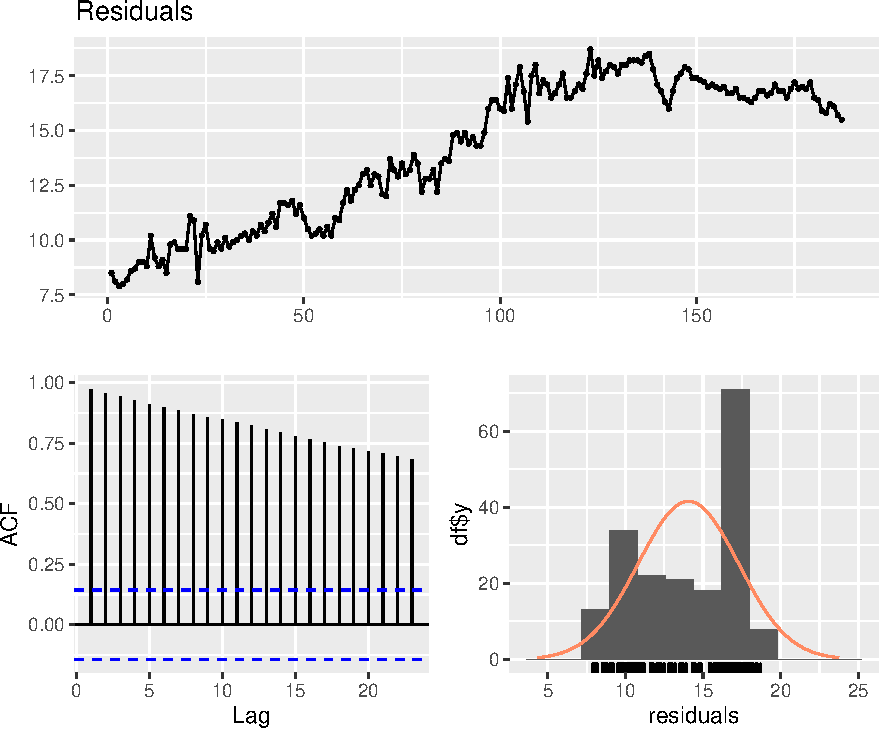
\includegraphics{TS_proj_files/figure-latex/unnamed-chunk-25-1.pdf}

\hypertarget{conclusion}{%
\section{Conclusion}\label{conclusion}}

\newpage

\hypertarget{reference-list}{%
\section{Reference List}\label{reference-list}}

Du Plessis, S., Smit, B. and Sturzenegger, F., 2008. Identifying
aggregate supply and demand shocks in South Africa. Journal of African
economies, 17(5), pp.765-793.

Ozcicek, O. Lag Length Selection in Vector Autoregressive Models:
Symmetric and Asymmetric Lags. Working Paper.
\url{https://www.lsu.edu/business/economics/files/workingpapers/pap97_27.pdf}

\newpage

\hypertarget{appendix}{%
\section{Appendix}\label{appendix}}

\hypertarget{forecast}{%
\subsection{Forecast}\label{forecast}}

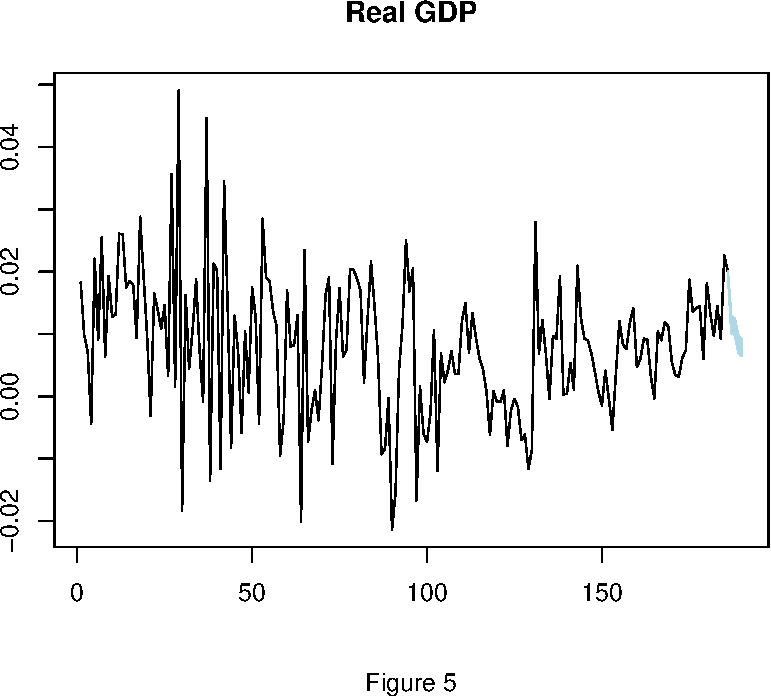
\includegraphics{TS_proj_files/figure-latex/unnamed-chunk-26-1.pdf}

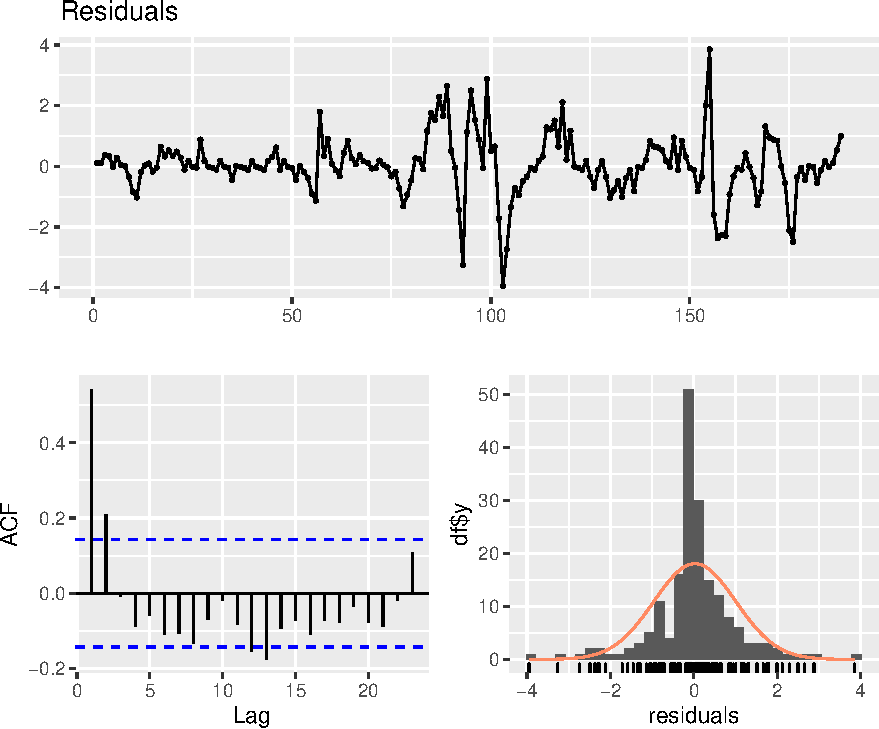
\includegraphics{TS_proj_files/figure-latex/unnamed-chunk-27-1.pdf}

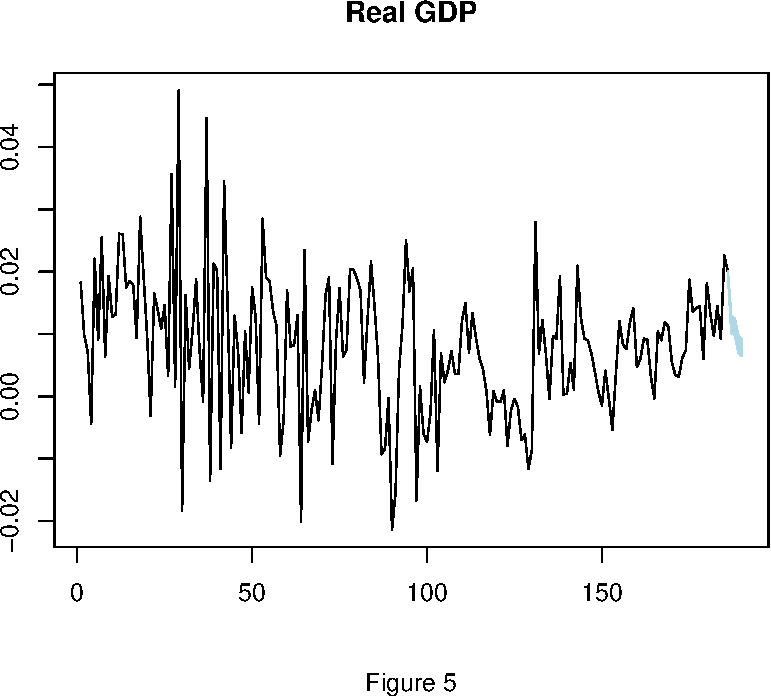
\includegraphics{TS_proj_files/figure-latex/unnamed-chunk-28-1.pdf}

\hypertarget{testing-for-stationarity}{%
\subsection{Testing for Stationarity}\label{testing-for-stationarity}}

\begin{verbatim}
## 
##  Augmented Dickey-Fuller Test
## 
## data:  real_gdp1
## Dickey-Fuller = -3.7922, Lag order = 5, p-value = 0.0208
## alternative hypothesis: stationary
\end{verbatim}

\begin{verbatim}
## 
##  Augmented Dickey-Fuller Test
## 
## data:  rg83
## Dickey-Fuller = -3.5737, Lag order = 4, p-value = 0.03979
## alternative hypothesis: stationary
\end{verbatim}

\begin{verbatim}
## 
##  Augmented Dickey-Fuller Test
## 
## data:  Real_interest1$Real_interest_rate
## Dickey-Fuller = -2.6335, Lag order = 5, p-value = 0.3112
## alternative hypothesis: stationary
\end{verbatim}

\begin{verbatim}
## 
##  Augmented Dickey-Fuller Test
## 
## data:  ri83$Real_interest_rate
## Dickey-Fuller = -2.7977, Lag order = 4, p-value = 0.2473
## alternative hypothesis: stationary
\end{verbatim}

\begin{verbatim}
## 
##  Augmented Dickey-Fuller Test
## 
## data:  ri_sa$seasonally_differenced
## Dickey-Fuller = -5.7783, Lag order = 5, p-value = 0.01
## alternative hypothesis: stationary
\end{verbatim}

\begin{verbatim}
## 
##  Augmented Dickey-Fuller Test
## 
## data:  g_g_not_s$Value
## Dickey-Fuller = -0.66065, Lag order = 5, p-value = 0.9724
## alternative hypothesis: stationary
\end{verbatim}

\begin{verbatim}
## 
##  Augmented Dickey-Fuller Test
## 
## data:  gg83$Value
## Dickey-Fuller = -2.3567, Lag order = 4, p-value = 0.4292
## alternative hypothesis: stationary
\end{verbatim}

\hypertarget{lag-selection-impulse-response-functions}{%
\subsection{Lag Selection Impulse Response
Functions}\label{lag-selection-impulse-response-functions}}

The set of Impulse Response Functions presented below are created using
a second SVAR model, where the number of lags selected is 6.

Impulse Response of the real GDP for each of the identified shocks:

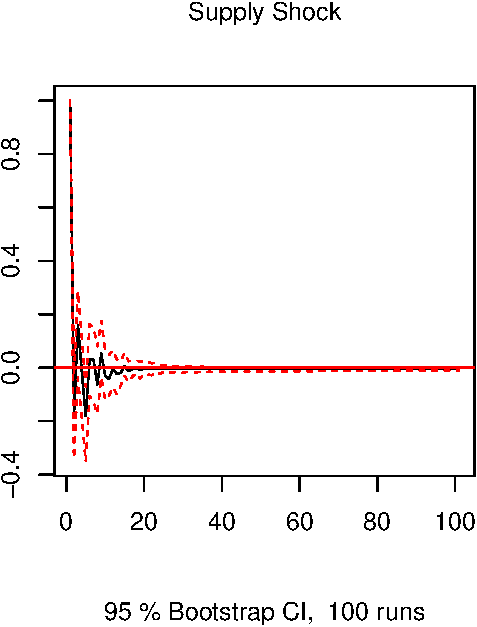
\includegraphics{TS_proj_files/figure-latex/unnamed-chunk-30-1.pdf}
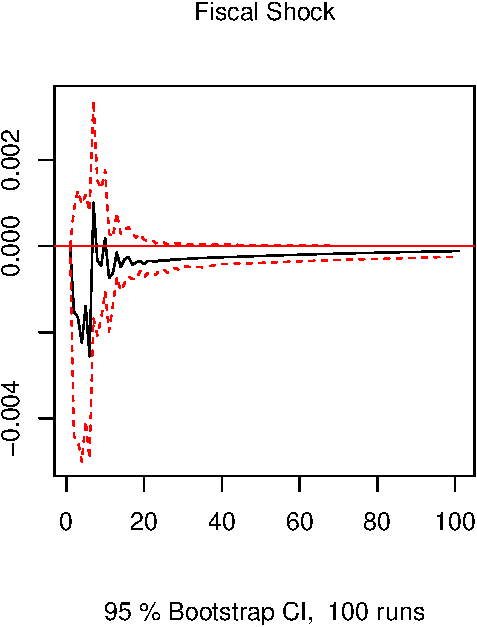
\includegraphics{TS_proj_files/figure-latex/unnamed-chunk-30-2.pdf}
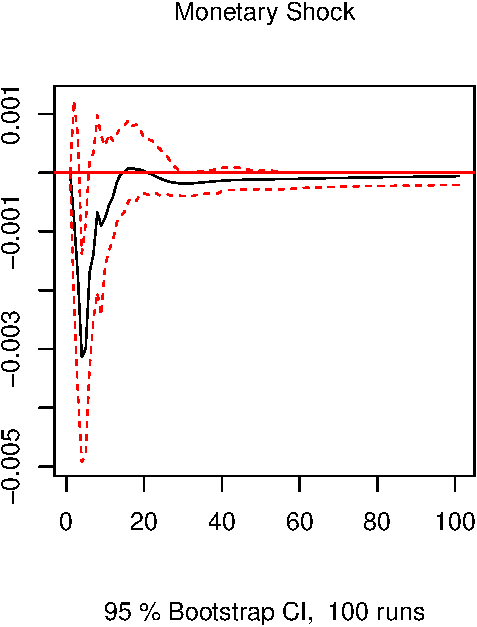
\includegraphics{TS_proj_files/figure-latex/unnamed-chunk-30-3.pdf}

Impulse Response of the real interest rate for each of the identified
shocks:

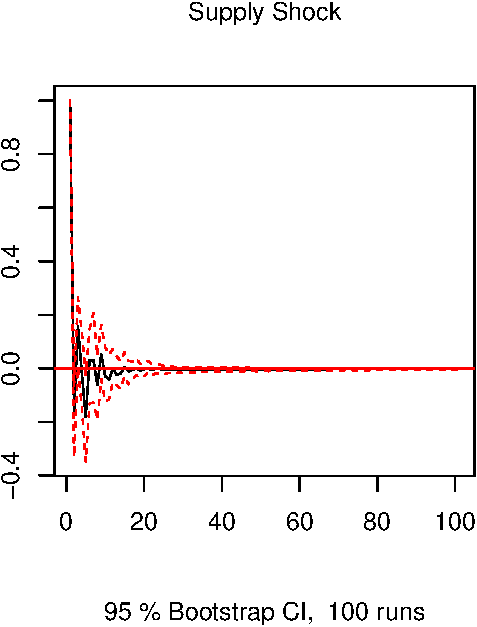
\includegraphics{TS_proj_files/figure-latex/unnamed-chunk-31-1.pdf}
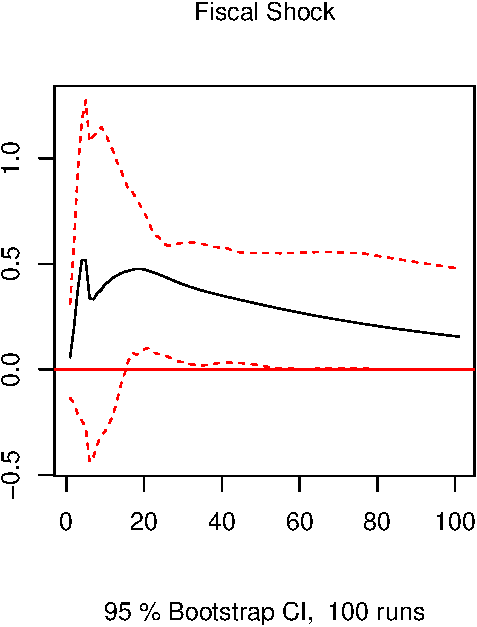
\includegraphics{TS_proj_files/figure-latex/unnamed-chunk-31-2.pdf}
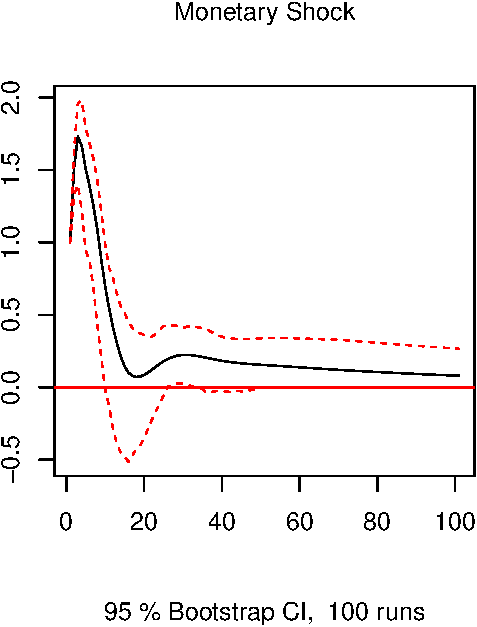
\includegraphics{TS_proj_files/figure-latex/unnamed-chunk-31-3.pdf}

Impulse Response of the government consumption to real GDP for each of
the identified shocks:

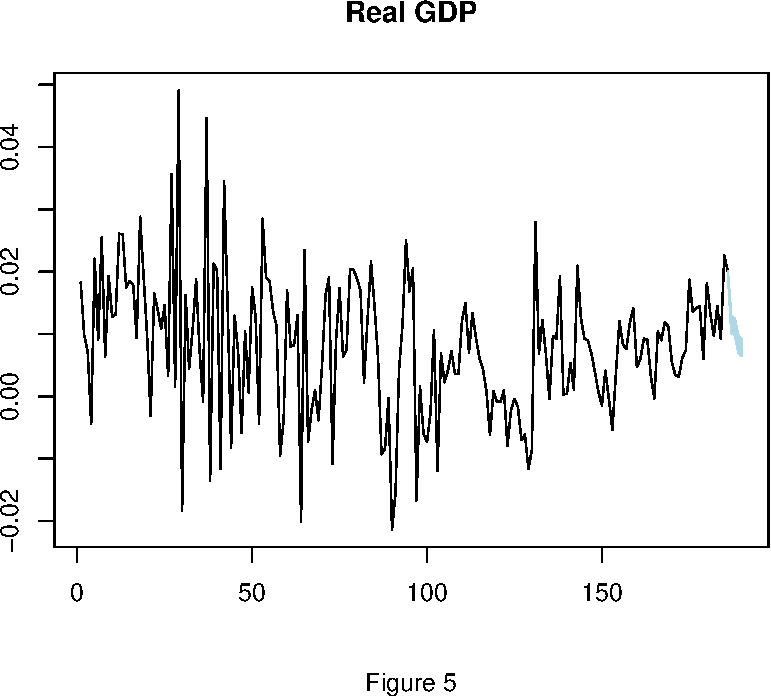
\includegraphics{TS_proj_files/figure-latex/unnamed-chunk-32-1.pdf}
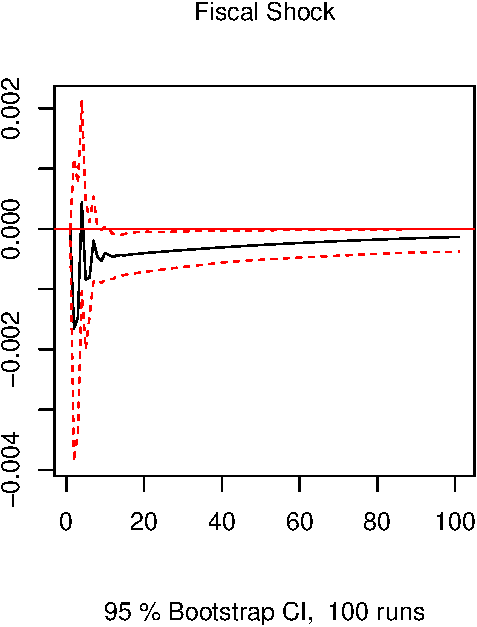
\includegraphics{TS_proj_files/figure-latex/unnamed-chunk-32-2.pdf}
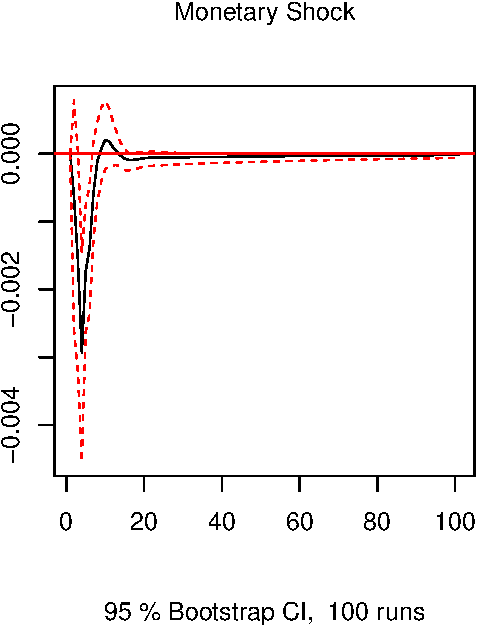
\includegraphics{TS_proj_files/figure-latex/unnamed-chunk-32-3.pdf}

The set of Impulse Response Functions presented below are created using
a third SVAR model, where the number of lags selected is 2.

Impulse Response of the real GDP for each of the identified shocks:

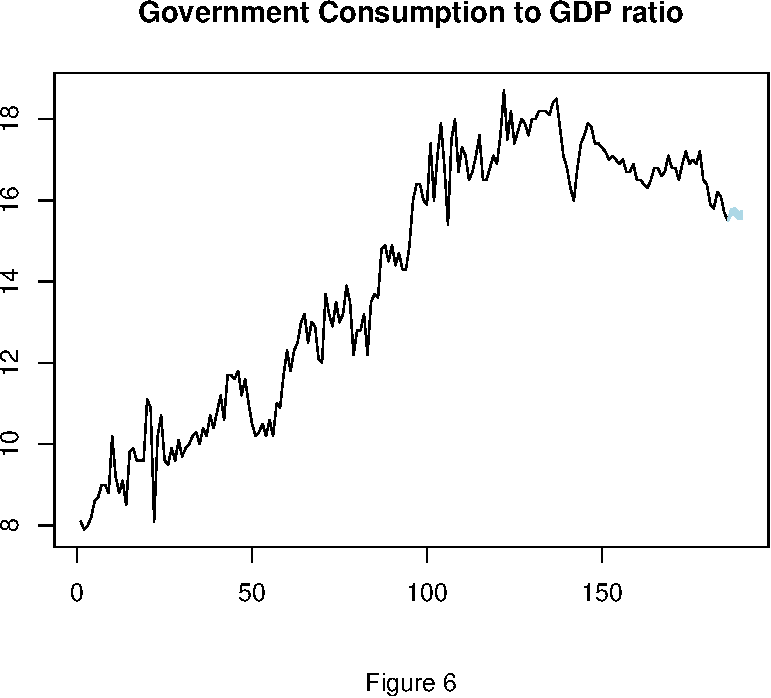
\includegraphics{TS_proj_files/figure-latex/unnamed-chunk-33-1.pdf}
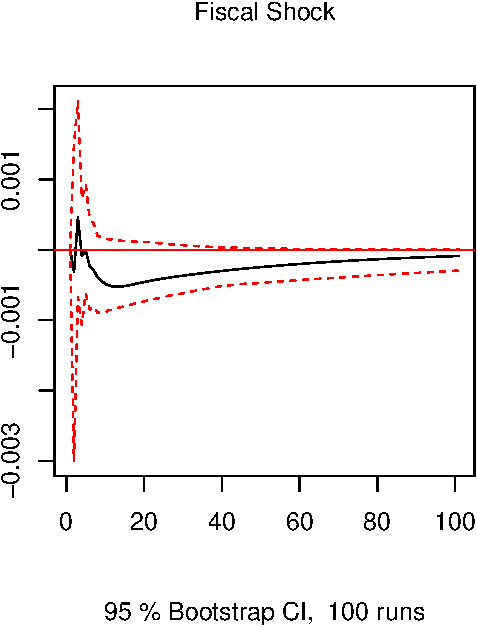
\includegraphics{TS_proj_files/figure-latex/unnamed-chunk-33-2.pdf}
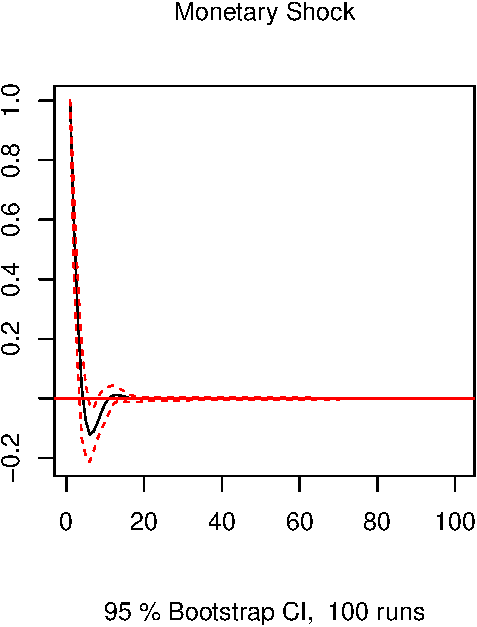
\includegraphics{TS_proj_files/figure-latex/unnamed-chunk-33-3.pdf}

Impulse Response of the real interest rate for each of the identified
shocks:

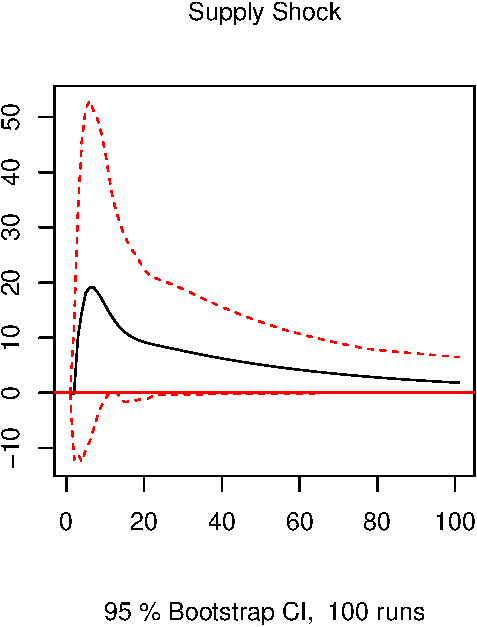
\includegraphics{TS_proj_files/figure-latex/unnamed-chunk-34-1.pdf}
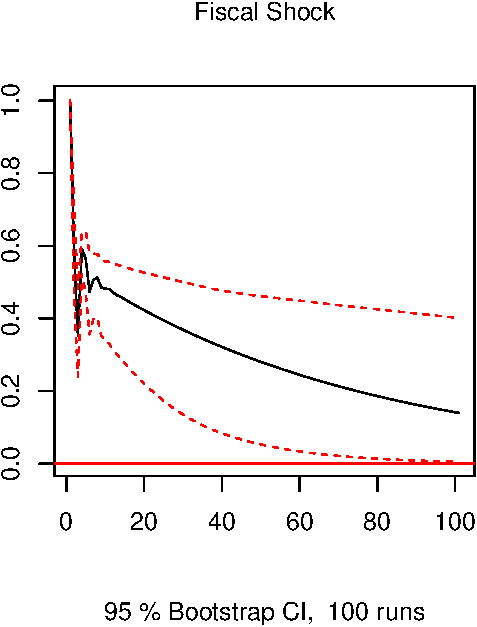
\includegraphics{TS_proj_files/figure-latex/unnamed-chunk-34-2.pdf}
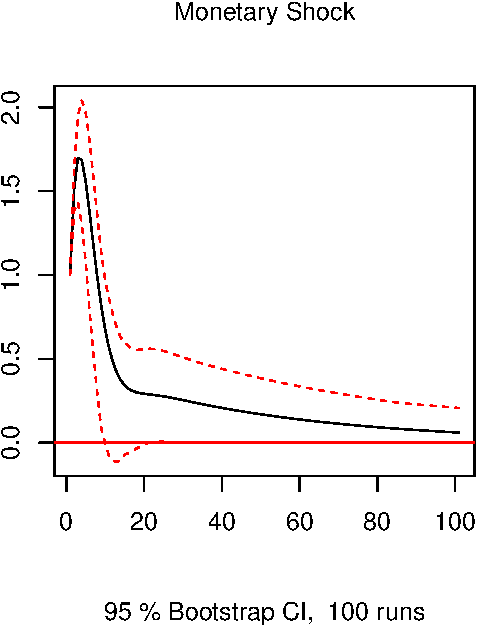
\includegraphics{TS_proj_files/figure-latex/unnamed-chunk-34-3.pdf}

Impulse Response of the government consumption to real GDP for each of
the identified shocks:

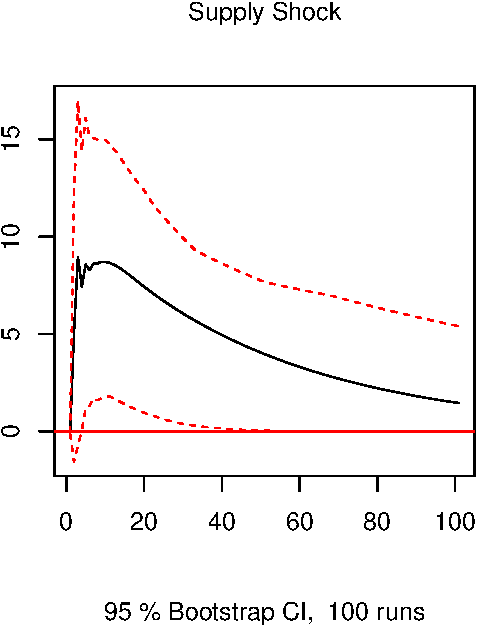
\includegraphics{TS_proj_files/figure-latex/unnamed-chunk-35-1.pdf}
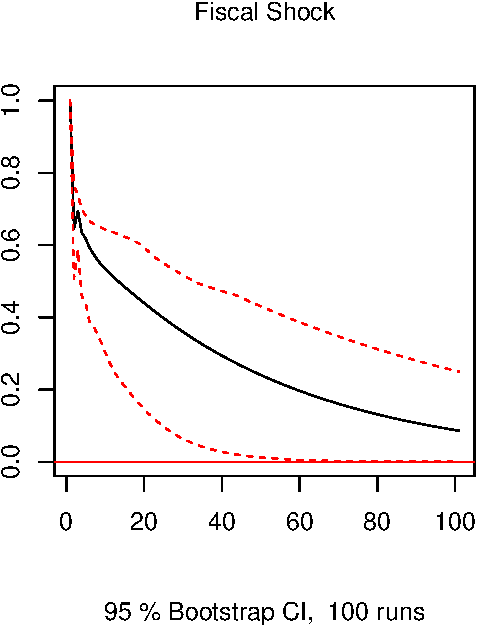
\includegraphics{TS_proj_files/figure-latex/unnamed-chunk-35-2.pdf}
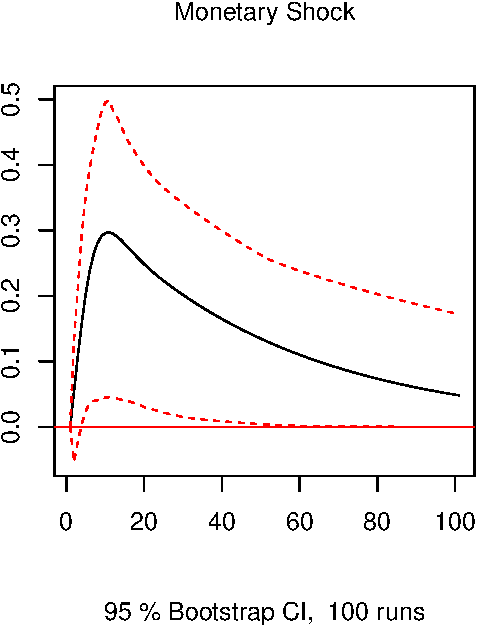
\includegraphics{TS_proj_files/figure-latex/unnamed-chunk-35-3.pdf}

\hypertarget{reduced-sample-impulse-response-functions}{%
\subsection{Reduced Sample Impulse Response
Functions}\label{reduced-sample-impulse-response-functions}}

Impulse Response of real GDP for each of the identified shocks:

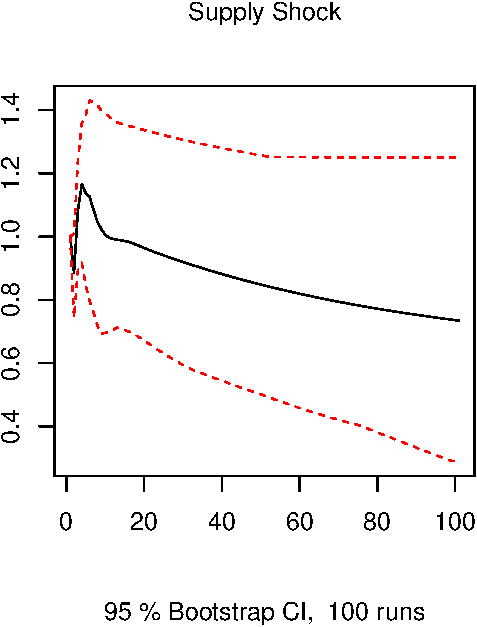
\includegraphics{TS_proj_files/figure-latex/unnamed-chunk-36-1.pdf}
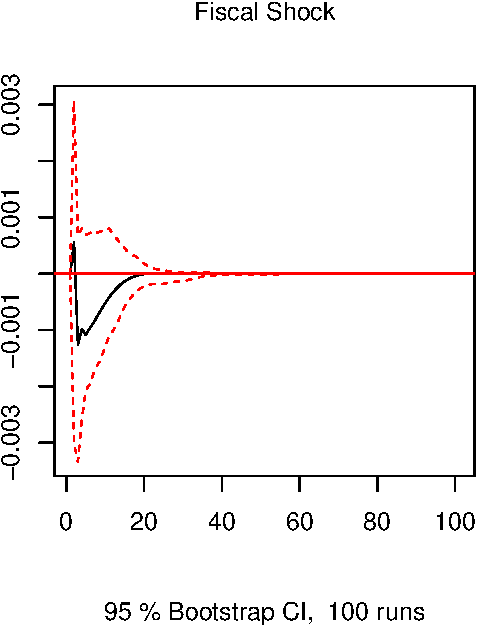
\includegraphics{TS_proj_files/figure-latex/unnamed-chunk-36-2.pdf}
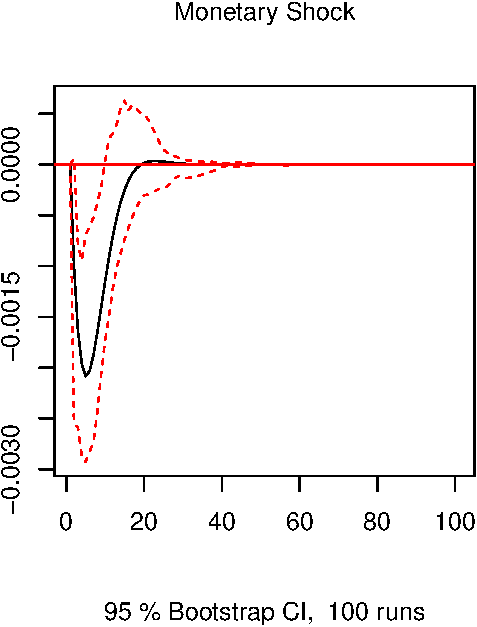
\includegraphics{TS_proj_files/figure-latex/unnamed-chunk-36-3.pdf}

Impulse Response of the real interest rate for each of the identified
shocks:

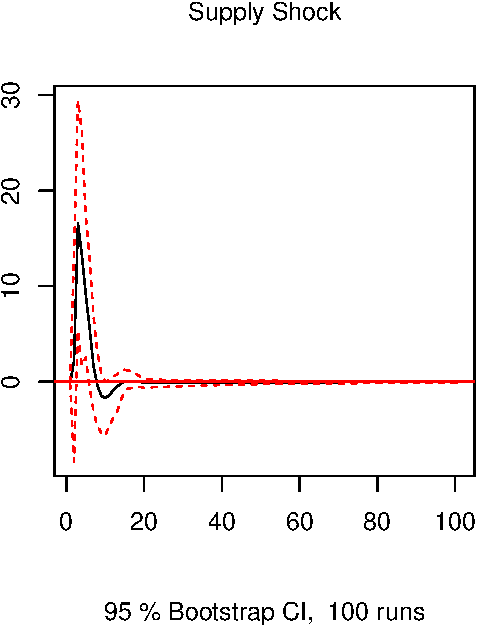
\includegraphics{TS_proj_files/figure-latex/unnamed-chunk-37-1.pdf}
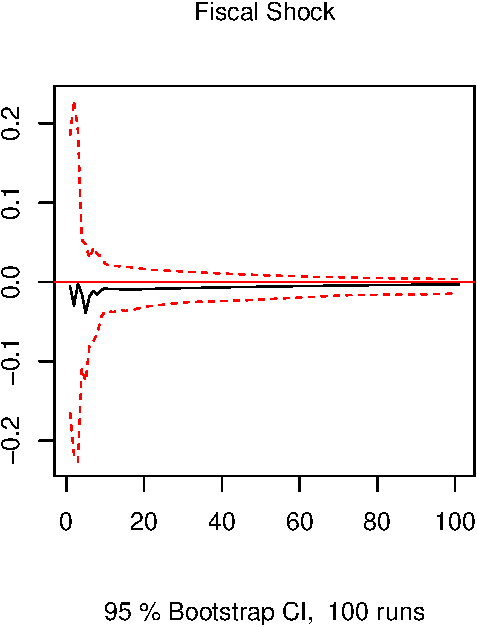
\includegraphics{TS_proj_files/figure-latex/unnamed-chunk-37-2.pdf}
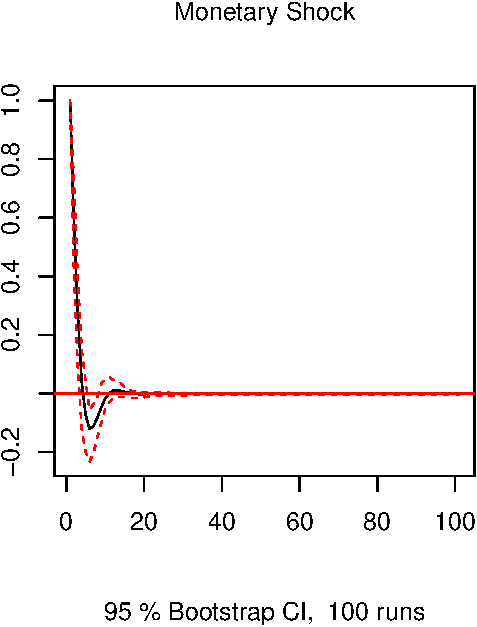
\includegraphics{TS_proj_files/figure-latex/unnamed-chunk-37-3.pdf}

Impulse Response of the government consumption to real GDP for each of
the identified shocks:

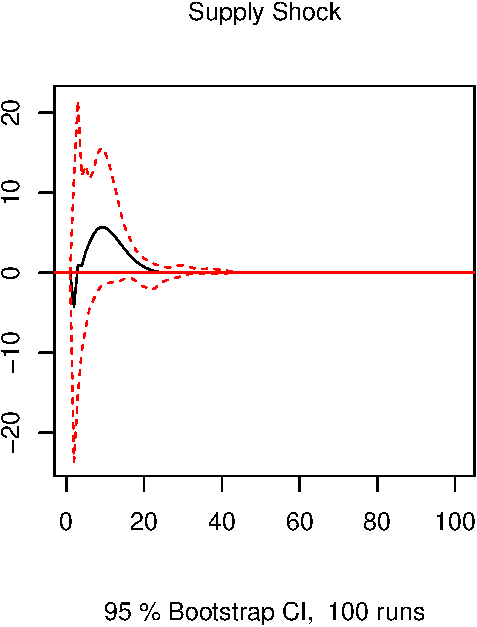
\includegraphics{TS_proj_files/figure-latex/unnamed-chunk-38-1.pdf}
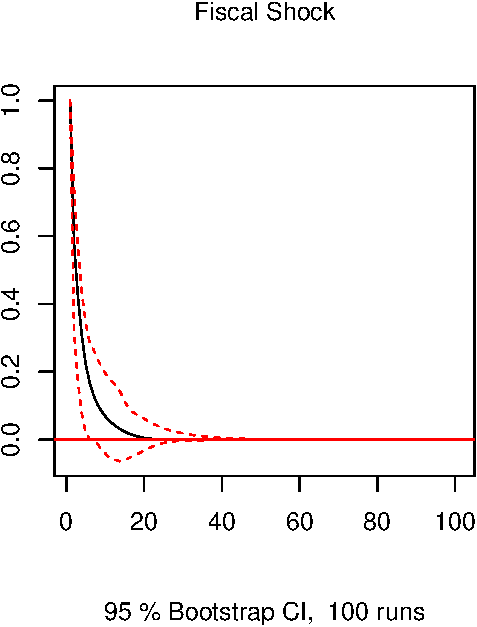
\includegraphics{TS_proj_files/figure-latex/unnamed-chunk-38-2.pdf}
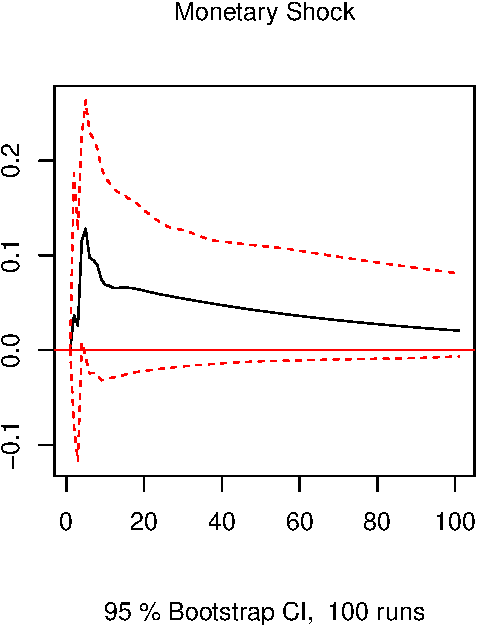
\includegraphics{TS_proj_files/figure-latex/unnamed-chunk-38-3.pdf}

\hypertarget{removing-seasonality-and-non-stationarity-impulse-response-functions}{%
\subsection{Removing Seasonality and Non-stationarity Impulse Response
Functions}\label{removing-seasonality-and-non-stationarity-impulse-response-functions}}

Impulse Response of real GDP for each of the identified shocks:

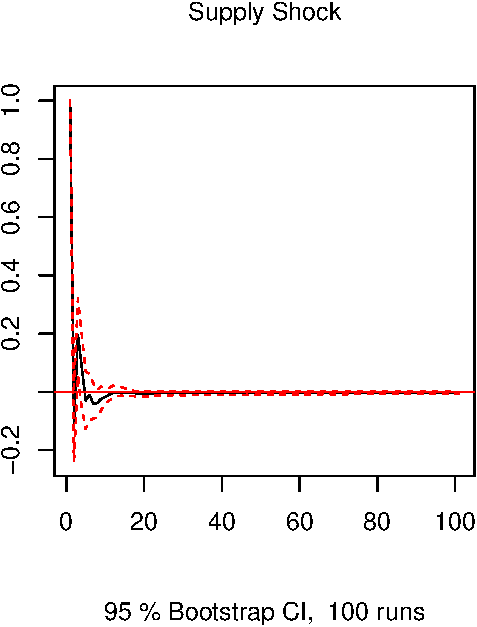
\includegraphics{TS_proj_files/figure-latex/unnamed-chunk-39-1.pdf}
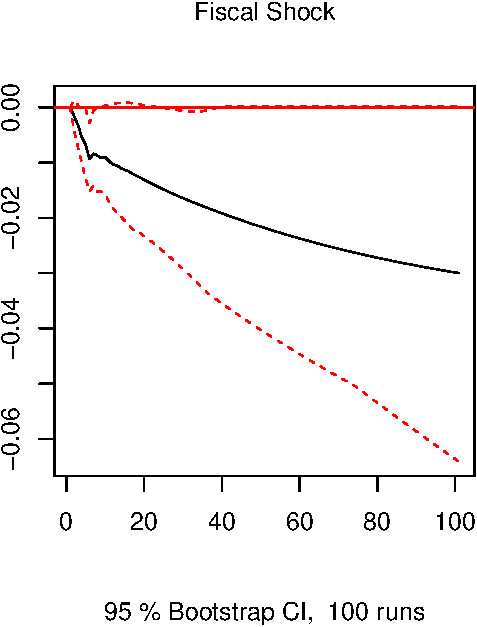
\includegraphics{TS_proj_files/figure-latex/unnamed-chunk-39-2.pdf}
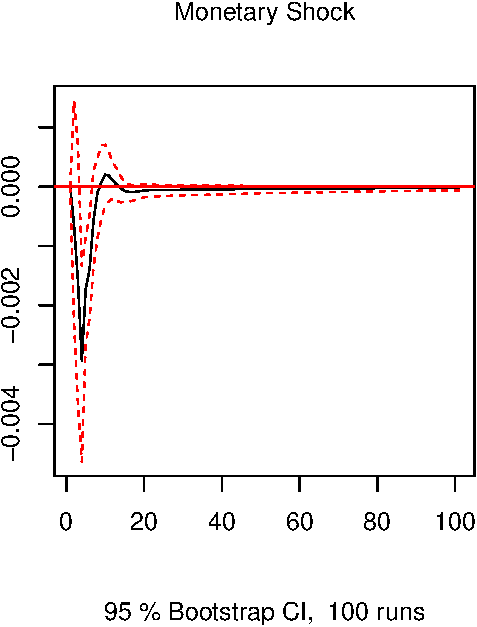
\includegraphics{TS_proj_files/figure-latex/unnamed-chunk-39-3.pdf}

Impulse Response of the real interest rate for each of the identified
shocks:

\includegraphics{TS_proj_files/figure-latex/unnamed-chunk-40-1.pdf}
\includegraphics{TS_proj_files/figure-latex/unnamed-chunk-40-2.pdf}
\includegraphics{TS_proj_files/figure-latex/unnamed-chunk-40-3.pdf}

Impulse Response of the government consumption to real GDP for each of
the identified shocks:

\includegraphics{TS_proj_files/figure-latex/unnamed-chunk-41-1.pdf}
\includegraphics{TS_proj_files/figure-latex/unnamed-chunk-41-2.pdf}
\includegraphics{TS_proj_files/figure-latex/unnamed-chunk-41-3.pdf}

\bibliography{Tex/ref}





\end{document}
